\titlespacing{\chapter}{0pt}{120pt}{7pt}
\chapter{Análisis de la situación Actual}
\label{cap:metodologia}
\authoredby{B}

\section{Diagrama del proceso, mapa del flujo de valor y/o diagrama de operacón actual}

\textbf{Diagrama del proceso}

A continuación, se presenta un diagrama de flujo que ilustra el proceso de visita a la página web de Proefex. Este diagrama ofrece una representación visual del flujo de acciones que un usuario podría llevar a cabo al interactuar con el sitio web de la empresa.

El propósito de este diagrama es proporcionar una comprensión clara y concisa del recorrido típico de un visitante en el sitio web de Proefex, desde el inicio de la visita hasta el posible contacto con la empresa para obtener más información o servicios.

A través de esta representación gráfica, se busca destacar las etapas clave y las decisiones potenciales que un usuario puede enfrentar durante su interacción con la plataforma en línea de Proefex.

A continuación se muestra el diagrama de flujo:

\begin{figure}[!ht]
\centering
\tikzstyle{startstop} = [ellipse, draw, text width=3cm, text centered, minimum height=1cm]
\tikzstyle{process} = [rectangle, draw, text width=3cm, text centered, minimum height=1cm]
\tikzstyle{decision} = [diamond, draw, text width=3cm, text centered, minimum height=1cm]
\tikzstyle{arrow} = [-{Stealth[length=5mm,width=3mm]}, thick]

\begin{tikzpicture}[node distance=3.5cm, auto]
  \node [startstop] (start) {Inicio};
  \node [process, below of=start] (visit) {Visitar el sitio web de Proefex};
  \node [decision, below of=visit] (interested) {¿Interesado en servicios?};
  \node [process, below of=interested, yshift=-0.5cm] (explore) {Explorar servicios ofrecidos};
  \node [decision, below of=explore, yshift=-0.5cm] (contact) {¿Desea contactar?};
  \node [process, below of=contact, yshift=-0.5cm] (contactinfo) {Obtener información de contacto};
  \node [startstop, below of=contactinfo] (end) {Fin};

  \draw [arrow] (start) -- (visit);
  \draw [arrow] (visit) -- (interested);
  \draw [arrow] (interested) -- node[anchor=east] {Sí} (explore);
  \draw [arrow] (interested) -| node[anchor=south] {No}  ++(3,-3) |- (end);
  \draw [arrow] (explore) -- (contact);
  \draw [arrow] (contact) -- node[anchor=east] {Sí} (contactinfo);
  \draw [arrow] (contact) -| node[anchor=south] {No} ++(-3,-3) |- (end);
  \draw [arrow] (contactinfo) -- (end);
\end{tikzpicture}
\end{figure}

\newpage
\textbf{diagrama de operación}

El diagrama de operación presentado a continuación representa el flujo de interacción de un usuario al navegar por la página web de Proefex. Este diagrama se ha creado con el propósito de visualizar de manera clara y concisa las secciones principales a las que un usuario puede acceder durante su visita al sitio web de la empresa.

Las secciones representadas en el diagrama incluyen Inicio, Servicios, Eventos, Nosotros, Contacto, Blog y Recursos. Cada una de estas secciones desempeña un papel fundamental en la experiencia del usuario al proporcionar información, servicios, eventos, contacto con la empresa, contenido del blog y acceso a recursos adicionales respectivamente.

El flujo de operación mostrado en el diagrama refleja el recorrido esperado de un usuario al explorar las diversas secciones del sitio web de Proefex. Se busca destacar la navegación intuitiva y la conectividad entre las secciones, permitiendo al usuario moverse de manera fluida y lógica a través del contenido proporcionado por la empresa.

\begin{figure}[!ht]
\centering
\tikzstyle{circleblock} = [circle, draw, text width=1.5cm, text centered, minimum height=1.5cm]
\tikzstyle{squareblock} = [rectangle, draw, text width=1.5cm, text centered, minimum height=1.5cm]
\tikzstyle{line} = [-{Stealth[length=5mm,width=3mm]}, thick]

\begin{tikzpicture}[node distance=3cm, auto]
  \node [circleblock] (inicio) {Inicio};
  \node [circleblock, right of=inicio] (servicios) {Servicios};
  \node [circleblock, below of=servicios] (eventos) {Eventos};
  \node [circleblock, below of=inicio] (nosotros) {Nosotros};
  \node [circleblock, below of=nosotros] (contacto) {Contacto};
  \node [circleblock, below of=contacto] (blog) {Blog};
  \node [squareblock, right of=servicios, xshift=1.5cm] (recursos) {Recursos};

  \draw [line] (inicio) -- (servicios);
  \draw [line] (servicios) -- (eventos);
  \draw [line] (eventos) -- (nosotros);
  \draw [line] (nosotros) -- (contacto);
  \draw [line] (contacto) -- (blog);
  \draw [line] (blog) -- (recursos);
  \draw [line] (recursos) -- (servicios);
\end{tikzpicture}
\end{figure}

\newpage
\section{Efectos del problema en el área de trabajo o en los resultados de la empresa}

La limitada interacción y el enfoque estático en la presentación de servicios a 
través de texto e imágenes en la página web de Proefex pudo haber generado ciertos 
efectos en la experiencia del usuario y en los resultados de la empresa:

\begin{itemize}
\item \textbf{Limitación en la comprensión}

El enfoque estático puede haber dificultado la comprensión completa de los servicios
ofrecidos, ya que las descripciones visuales podrían no haber sido lo suficientemente
explícitas o atractivas.

\item \textbf{Posible Pérdida de Clientes Potenciales}

La falta de elementos interactivos y visuales atractivos podría haber reducido la
retención de visitantes y, por ende, la conversión de clientes potenciales.

\item \textbf{Menor Diferenciación de la Competencia}

Una presentación estática de servicios puede haber afectado la diferenciación
de Proefex respecto a sus competidores, limitando la percepción de innovación
y modernización.

\item \textbf{Menor Impacto de Marketing}

La falta de elementos visuales interactivos podría haber reducido el impacto del
marketing en línea, limitando el alcance y la efectividad de las campañas.

\end{itemize}

\section{Análisis de las causas raíces que generan el problema}

El problema identificado en la presentación estática de servicios en la página
web de Proefex puede tener múltiples causas subyacentes que han contribuido a
esta limitación en la interactividad y medios visuales dinámicos. Las posibles
causas raíces podrían ser:

\begin{itemize}
\item \textbf{Cultura Empresarial Conservadora}

Una mentalidad arraigada en presentaciones estáticas tradicionales, lo que ha
limitado la adopción de métodos más interactivos y visuales.

\item \textbf{Recursos Limitados para el Desarrollo}

Limitaciones presupuestarias o de recursos que han impedido la inversión en
herramientas o personal especializado en desarrollo interactivo.

\end{itemize}

\section{Priorización de causas raíces}

\begin{enumerate}
\item \textbf{Impacto en el Problema}
Evaluar la magnitud del efecto de cada causa raíz en la limitación de la interactividad
y presentación de servicios en la página web de Proefex.

\item \textbf{Frecuencia de Aparición}
Determinar con qué frecuencia o en qué medida cada causa raíz contribuye al problema.

\item \textbf{Factibilidad de Solución}
Evaluar la factibilidad de la solución actual para solucionar el problema.

\begin{table}[!ht]
\begin{center}
\begin{tabular}{| p{4cm} | p{3cm} | p{2cm} | p{2cm} | p{2cm} | }
\hline
Causa Raiz & Impacto en el Problema & Frecuencia & Factibilidad & Puntuación total \\ \hline
Cultura Empresarial Conservadora & Alta & Media & Alta & 8 \\ \hline
Recursos Limitados para el Desarrollo & Alta & Alta & Media & 9 \\ \hline
\end{tabular}

\caption{Priorización de causas raíces}
\label{tab:causasraiz}
\end{center}
\end{table} 
\end{enumerate}

\begin{figure}[ht]
  \centering
  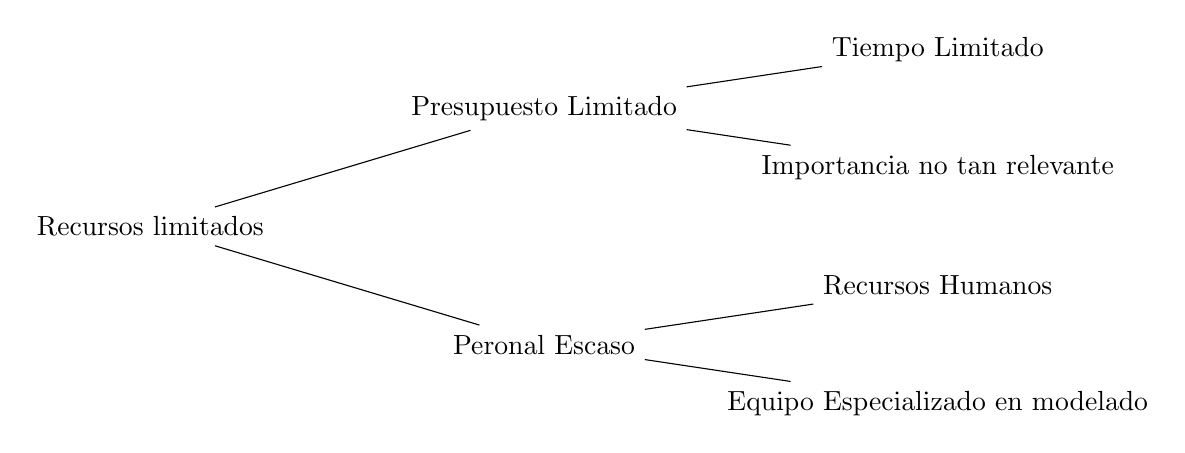
\begin{tikzpicture}[
    level/.style={sibling distance=3cm/#1, level distance=5cm},
    grow=right
  ]
    \node {Recursos limitados}
      child {
        node {Peronal Escaso}
        child { node {Equipo Especializado en modelado} }
        child { node {Recursos Humanos} } 
      }
      child {
        node {Presupuesto Limitado}
        child { node {Importancia no tan relevante} }
        child { node {Tiempo Limitado} }
      };
  \end{tikzpicture}
  \caption{Sub-causas de Limitaciones Tecnológicas o de Recursos.}
\end{figure}

En esta sección, analizaremos de forma gráfica el problema mediante el Diagrama
de Pareto para identificar las áreas clave de enfoque. Este método nos permite
priorizar las limitaciones más significativas, optimizar recursos y diseñar
estrategias efectivas para mejorar la presentación de servicios mediante la
interactividad con modelos 2D y animaciones.

% Tabla de problemas y puntuaciones
\begin{table}[ht]
  \centering
  \caption{Descripción de Problemas y Puntuaciones}
  \begin{tabularx}{0.8\linewidth}{X c}
    \toprule
    \textbf{Problema} & \textbf{Puntuación} \\
    \midrule
    Falta de personal especializado en modelado & 80 \\
    Tiempo de inversión limitado & 65 \\
    Escasez de recursos económicos & 50 \\
    \bottomrule
  \end{tabularx}
\end{table}

% Tabla de causas y valoraciones
\begin{table}[ht]
  \centering
  \caption{Causas y Valoraciones}
  \begin{tabularx}{0.8\linewidth}{X c}
    \toprule
    \textbf{Causa} & \textbf{Valoración} \\
    \midrule
    Limitaciones de Recursos & 80 \\
    Limitaciones de Tiempo & 65 \\
    Restricciones Económicas & 50 \\
    \bottomrule
  \end{tabularx}
\end{table}



\begin{figure}[ht]
  \centering
  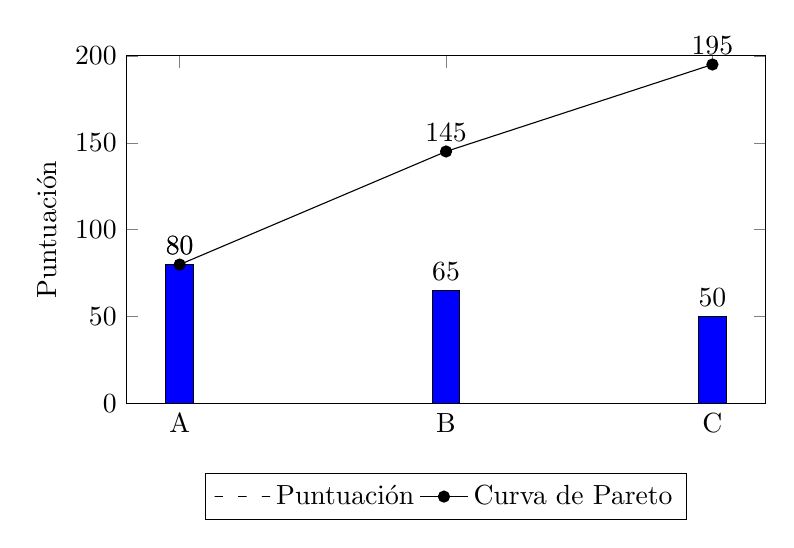
\begin{tikzpicture}
    \begin{axis}[
      ylabel=Puntuación,
      width=0.8\textwidth,
      height=6cm,
      ymin=0,
      ymax=200,
      xtick=data,
      symbolic x coords={A, B, C},
      xticklabels={A, B, C},
      nodes near coords,
      legend style={at={(0.5,-0.2)},anchor=north,legend columns=-1},
    ]
    \addplot[ybar,fill=blue] 
      coordinates {(A,80) (B,65) (C,50)};
    %
    \addplot[draw,mark=*] 
      coordinates {(A,80) (B,145) (C,195)};
    \legend{Puntuación, Curva de Pareto}
	% Leyenda en el gráfico
    \end{axis}
  \end{tikzpicture}
  \caption{Diagrama de Pareto con Curva de Distribución Acumulada.}
\end{figure}

\textbf{Leyenda:}
A: Limitaciones de Recursos \\
B: Limitaciones de Tiempo \\
C: Restricciones Económicas

\newpage

El resultado del Diagrama de Pareto nos muestra claramente las limitaciones más
relevantes que afectan la presentación de servicios con modelos 2D y animaciones
en Proefex. Al analizar este gráfico, se identifican las áreas prioritarias para
enfocar nuestros esfuerzos de mejora.

En términos de interpretación, las barras representan la magnitud de cada limitación
específica, permitiéndonos ver claramente cuáles tienen el mayor impacto. La curva
acumulada nos muestra la contribución acumulada de cada limitación, evidenciando 
las áreas que representan la mayor proporción del problema.

En este sentido, las limitaciones identificadas en los primeros lugares del 
gráfico (las barras más altas y la mayor contribución acumulada) son las áreas 
críticas que requieren atención inmediata para mejorar la presentación de
servicios. Esto nos guía en la asignación estratégica de recursos y esfuerzos
para abordar efectivamente los desafíos más relevantes.

